% THIS DOCUMENT IS TAILORED TO REQUIREMENTS FOR SCIENTIFIC COMPUTING.  IT SHOULDN'T
% BE USED FOR NON-SCIENTIFIC COMPUTING PROJECTS
\documentclass[12pt]{article}

\usepackage{amsmath, mathtools}
\usepackage{amsfonts}
\usepackage{amssymb}
\usepackage{graphicx}
\usepackage{colortbl}
\usepackage{xr}
\usepackage{hyperref}
\usepackage{longtable}
\usepackage{xfrac}
\usepackage{tabularx}
\usepackage{float}
\usepackage{siunitx}
\usepackage{booktabs}
\usepackage{caption}
\usepackage{pdflscape}
\usepackage{afterpage}
\usepackage{tikz}
\usetikzlibrary{shapes.geometric, arrows}
\usepackage{graphicx}
\graphicspath{{./images/}}
\usepackage[round]{natbib}

%\usepackage{refcheck}

\hypersetup{
    bookmarks=true,         % show bookmarks bar?
      colorlinks=true,       % false: boxed links; true: colored links
    linkcolor=red,          % color of internal links (change box color with linkbordercolor)
    citecolor=green,        % color of links to bibliography
    filecolor=magenta,      % color of file links
    urlcolor=cyan           % color of external links
}

%% Comments

\usepackage{color}

\newif\ifcomments\commentstrue %displays comments
%\newif\ifcomments\commentsfalse %so that comments do not display

\ifcomments
\newcommand{\authornote}[3]{\textcolor{#1}{[#3 ---#2]}}
\newcommand{\todo}[1]{\textcolor{red}{[TODO: #1]}}
\else
\newcommand{\authornote}[3]{}
\newcommand{\todo}[1]{}
\fi

\newcommand{\wss}[1]{\authornote{blue}{SS}{#1}} 
\newcommand{\plt}[1]{\authornote{magenta}{TPLT}{#1}} %For explanation of the template
\newcommand{\an}[1]{\authornote{cyan}{Author}{#1}}

%% Common Parts

\newcommand{\progname}{ProgName} % PUT YOUR PROGRAM NAME HERE
\newcommand{\authname}{Team \#, Team Name
\\ Student 1 name
\\ Student 2 name
\\ Student 3 name
\\ Student 4 name} % AUTHOR NAMES                  

\usepackage{hyperref}
    \hypersetup{colorlinks=true, linkcolor=blue, citecolor=blue, filecolor=blue,
                urlcolor=blue, unicode=false}
    \urlstyle{same}
                                


% For easy change of table widths
\newcommand{\colZwidth}{1.0\textwidth}
\newcommand{\colAwidth}{0.13\textwidth}
\newcommand{\colBwidth}{0.82\textwidth}
\newcommand{\colCwidth}{0.1\textwidth}
\newcommand{\colDwidth}{0.05\textwidth}
\newcommand{\colEwidth}{0.8\textwidth}
\newcommand{\colFwidth}{0.17\textwidth}
\newcommand{\colGwidth}{0.5\textwidth}
\newcommand{\colHwidth}{0.28\textwidth}

% Used so that cross-references have a meaningful prefix
\newcounter{defnum} %Definition Number
\newcommand{\dthedefnum}{GD\thedefnum}
\newcommand{\dref}[1]{GD\ref{#1}}
\newcounter{datadefnum} %Datadefinition Number
\newcommand{\ddthedatadefnum}{DD\thedatadefnum}
\newcommand{\ddref}[1]{DD\ref{#1}}
\newcounter{theorynum} %Theory Number
\newcommand{\tthetheorynum}{TM\thetheorynum}
\newcommand{\tref}[1]{TM\ref{#1}}
\newcounter{tablenum} %Table Number
\newcommand{\tbthetablenum}{TB\thetablenum}
\newcommand{\tbref}[1]{TB\ref{#1}}
\newcounter{assumpnum} %Assumption Number
\newcommand{\atheassumpnum}{A\theassumpnum}
\newcommand{\aref}[1]{A\ref{#1}}
\newcounter{goalnum} %Goal Number
\newcommand{\gthegoalnum}{GS\thegoalnum}
\newcommand{\gsref}[1]{GS\ref{#1}}
\newcounter{instnum} %Instance Number
\newcommand{\itheinstnum}{IM\theinstnum}
\newcommand{\iref}[1]{IM\ref{#1}}
\newcounter{reqnum} %Requirement Number
\newcommand{\rthereqnum}{R\thereqnum}
\newcommand{\rref}[1]{R\ref{#1}}
\newcounter{consnum} %Constraint Number
\newcommand{\rtheconsnum}{C\theconsnum}
\newcommand{\cref}[1]{C\ref{#1}}
\newcounter{psysnum} %Physical System Number
\newcommand{\rthepsysnum}{C\thepsysnum}
\newcommand{\psref}[1]{PS\ref{#1}}
\newcounter{nfrnum} %NFR Number
\newcommand{\rthenfrnum}{NFR\thenfrnum}
\newcommand{\nfrref}[1]{NFR\ref{#1}}
\newcounter{lcnum} %Likely change number
\newcommand{\lthelcnum}{LC\thelcnum}
\newcommand{\lcref}[1]{LC\ref{#1}}
\newcounter{rnnum} %Likely change number
\newcommand{\lthernnum}{RN\thernnum}
\newcommand{\rnref}[1]{RN\ref{#1}}
\newcounter{ulcnum} %Likely change number
\newcommand{\ltheulcnum}{ULC\theulcnum}
\newcommand{\ulcref}[1]{ULC\ref{#1}}
\newcommand{\ProjectName}{ESF }

\usepackage{fullpage}

\newcommand{\deftheory}[9][Not Applicable]
{
\newpage
\noindent \rule{\textwidth}{0.5mm}

\paragraph{RefName: } \textbf{#2} \phantomsection 
\label{#2}

\paragraph{Label:} #3

\noindent \rule{\textwidth}{0.5mm}

\paragraph{Equation:}

#4

\paragraph{Description:}

#5

\paragraph{Notes:}

#6

\paragraph{Source:}

#7

\paragraph{Ref.\ By:}

#8

\paragraph{Preconditions for \hyperref[#2]{#2}:}
\label{#2_precond}

#9

\paragraph{Derivation for \hyperref[#2]{#2}:}
\label{#2_deriv}

#1

\noindent \rule{\textwidth}{0.5mm}

}

\tikzstyle{actor} = [circle, 
minimum width=1cm, 
minimum height=1cm,
text centered, 
draw=black, 
fill=white!30]

\tikzstyle{process} = [rectangle, 
minimum width=2cm, 
minimum height=1cm, 
text centered,
text width=2cm, 
draw=black, 
fill=white!30]

\tikzstyle{io} = [trapezium, 
trapezium stretches=true, % A later addition
trapezium left angle=70, 
trapezium right angle=110,
text width=2cm,  
minimum width=2cm, 
minimum height=1cm, text centered, 
draw=black, fill=white!30]

\begin{document}

\title{Software Requirements Specification for \ProjectName: Equivariant Sensor Fusion for Autonomous Driving Object Detection} 
\author{Alaap Grandhi}
\date{\today}
	
\maketitle

~\newpage

\pagenumbering{roman}

\tableofcontents

~\newpage

\section*{Revision History}

\begin{tabularx}{\textwidth}{p{3cm}p{2cm}X}
\toprule {\bf Date} & {\bf Version} & {\bf Notes}\\
\midrule
February 9, 2025 & 1.0 & Initial SRS draft/document.\\
\midrule
April 16, 2025 & 2.0 & Updated SRS according to comments.\\
\bottomrule
\end{tabularx}

~\newpage

\section{Reference Material}

This section records information for easy reference.

\subsection{Table of Units}

Throughout this document SI (Syst\`{e}me International d'Unit\'{e}s) is employed
as the unit system.  In addition to the basic units, several derived units are
used as described below.  For each unit, the symbol is given followed by a
description of the unit and the SI name.
~\newline

\renewcommand{\arraystretch}{1.2}
%\begin{table}[ht]
  \noindent \begin{tabular}{l l l} 
    \toprule		
    \textbf{symbol} & \textbf{unit} & \textbf{SI}\\
    \midrule 
    \si{\metre} & length & metre\\
    \bottomrule
  \end{tabular}
  %	\caption{Provide a caption}
%\end{table}

\subsection{Table of Symbols}

The table that follows summarizes the symbols used in this document along with
their units. The symbols are listed in alphabetical order.

\renewcommand{\arraystretch}{1.2}
%\noindent \begin{tabularx}{1.0\textwidth}{l l X}
\noindent \begin{longtable*}{l l p{12cm}} \toprule
\textbf{symbol} & \textbf{unit} & \textbf{description}\\
\midrule 
$f_x$ & $\mathbb{R}_{\geq0}$ pixels & The focal length of the given camera in the $x$ direction.
\\
$f_y$ & $\mathbb{R}_{\geq0}$ pixels & The focal length of the given camera in the $y$ direction.
\\
$c_x$ & $\mathbb{R}$ pixels & The principal point of the given camera in the $x$ direction.
\\
$c_y$ & $\mathbb{R}$ pixels & The principal point of the given camera in the $y$ direction.
\\
$s$ & $\mathbb{R}$ pixels & The skew of the given camera representing how far from perpendicular the $x$ and $y$ directions are.
\\
$\mathbf{K}$ & $\mathbb{R}^{3\times3}$ pixels & The intrinsic matrix of the given camera representing how 3D points are projected onto the 2D image plane.
\\
$n_p$ & $\mathbb{R}_{\geq0}$ & The number of pixels in a given input image.
\\
$\mathbf{P_i}$ & $\mathbb{R}^{2\times{}n_p}$ pixels & The set of $x$,$y$ coordinates for each of the $n_p$ pixels in a given image.
\\
$\mathbf{P_c}$ & $\mathbb{R}^{3\times{}n_p}$ m & The set of back-projected $x$,$y$,$z$ coordinates for each of the $n_p$ pixels in a given image. This is just $X_{c}$, $Y_{c}$, and $Z_{c}$ concatenated.
\\
$\mathbf{X_c}$ & $\mathbb{R}^{n_p}$ m & The set of back-projected $x$ coordinates for each of the $n_p$ pixels in a given image.
\\
$\mathbf{Y_c}$ & $\mathbb{R}^{n_p}$ m & The set of back-projected $y$ coordinates for each of the $n_p$ pixels in a given image.
\\
$\mathbf{Z_c}$ & $\mathbb{R}^{n_p}$ m & The set of back-projected $z$ coordinates for each of the $n_p$ pixels in a given image.
\\
$D$ & $\mathbb{R}^{3}\rightarrow{}\mathbb{R}^{3}$ & The distortion model of the given camera (accounts for lens effects).
\\
$\mathbf{P_w}$ & $\mathbb{R}^{3\times{}n_p}$ m & The set of back-projected, world reference frame $x$,$y$,$z$ coordinates for each of the $n_p$ pixels in a given image.
\\
$\mathbf{T_{c,w}}$ & $\mathbb{R}^{4\times{}4}$ & The extrinsics matrix that maps $x$,$y$,$z$ points from the given camera's frame of reference to the world reference frame.
\\ 
$\mathbf{R_{c,w}}$ & $\mathbb{R}^{3\times3}$ & The rotation matrix between the given camera's frame of reference and the world reference frame.
\\
$\mathbf{t_{c,w}}$ & $\mathbb{R}^{3}$ & The translation vector between the given camera's frame of reference and the world reference frame.
\\
$\mathbb{P}$ & $\mathbb{R}^{n_c}$ & A predicted probability distribution over the set of $n_c$ discrete classes.
\\
$\alpha_{gd}$ & $\mathbb{R}$ & A hyperparameter for gradient descent that controls how large each gradient update is.
\\
$L$ & $\mathbb{R}^{n_\theta}\rightarrow\mathbb{R}$ & A loss function that maps the parameters of a model to a single estimated loss value.
\\
$n_{\theta}$ & $\mathbb{R}_{\geq0}$ & The number of learnable parameters for a given model.
\\
$\mathbf{\theta}$ & $\mathbb{R}^{n_\theta}$ & The learnable parameters for a given model, where the number of parameters is $n_\theta$.
\\
$\mathit{TP}$ & $\mathbb{N}_{0}$ & The number of true positives for a given classification task. That is, the number of positive predictions that corresponded to positive ground truth.
\\
$\mathit{FP}$ & $\mathbb{N}_{0}$ & The number of false positives for a given classification task. That is, the number of positive predictions that corresponded to a negative ground truth.
\\
$\mathit{FN}$ & $\mathbb{N}_{0}$ & The number of false negatives for a given classification task. That is, the number of positive ground truths that were not predicted to be positive.
\\
$\mathbf{d_{c}}$ & $\mathbb{R}^{n_p}$ m & The estimated depth values for each of the pixels in a given image.
\\
$g$ & $\mathbb{R}_{\geq0}$ & The number of scalar values/parameters used to define a bounding box (dataset-dependent). For the nuScenes dataset, this is 10 corresponding to the 3D center position, height, width, length, and a quaternion angle representation. 
\\
$n_{b}$ & $\mathbb{R}_{\geq0}$ & The number of ground truth bounding boxes. 
\\
$n_{\hat{b}}$ & $\mathbb{R}_{\geq0}$ & The number of predicted bounding boxes. 
\\
$n_{c}$ & $\mathbb{R}_{\geq0}$ & The number of object classes (typically 3 corresponding to cars, pedestrians, and cyclists). 
\\
$\mathbf{B}$ & $\mathbb{R}^{g\times{}n_b}$ & The set of ground-truth bounding box attributes (i.e. center, height, width, etc.), where there are $n_b$ ground truth bounding boxes.
\\
$\mathbf{\hat{B}}$ & $\mathbb{R}^{g\times{}n_{\hat{b}}}$ & The set of predicted bounding box attributes, where there are $n_{\hat{b}}$ predicted bounding boxes.
\\
$\mathbf{\hat{C}_{\text{dist}}}$ & $\mathbb{R}^{n_c\times{}n_{\hat{b}}}$ & The set of predicted bounding box class probability distributions.
\\
$\mathbf{\hat{c}}$ & $\mathbb{N}_{0}^{n_{\hat{b}}}$ & The set of predicted bounding box classes.
\\
$\mathbf{c}$ & $\mathbb{N}_{0}^{n_b}$ & The set of ground truth bounding box classes.
\\
$\alpha_{fl}$ & $\mathbb{R}$ & A hyperparameter for controlling the influence of the focal loss term.
\\
$\gamma$ & $\mathbb{R}$ & A hyperparameter for controlling the effect of easy examples on the focal loss. In practice, this is class specific and is set to the inverse class frequency.
\\
$\beta_1$ & $\mathbb{R}$ & A hyperparameter for changing the inertia of the first moment in ADAM.
\\
$\beta_2$ & $\mathbb{R}$ & A hyperparameter for changing the inertia of the second moment in ADAM.
\\
$\tau_{IoU}$ & $\mathbb{R}$ & An IoU threshold that is used to determine whether a predicted and a ground truth bounding box sufficiently overlap to be considered paired.
\\
$h$ & $\mathbb{R}_{\geq0}$ & The height of a given input image. 
\\
$w$ & $\mathbb{R}_{\geq0}$ & The width of a given input image. 
\\
$n_{l}$ & $\mathbb{R}_{\geq0}$ & The number of points in an input lidar pointcloud. 
\\
$\mathcal{I}$ & $\mathbb{R}^{h\times{}w}$ & An input image with height $h$ and width $w$.
\\
$\mathcal{P}$ & $\mathbb{R}^{3\times{}n_l}$ & An input lidar pointcloud with $n_l$ points.
\\
\bottomrule
\end{longtable*}

\subsection{Abbreviations and Acronyms}

\renewcommand{\arraystretch}{1.2}
\begin{tabular}{l l} 
  \toprule		
  \textbf{symbol} & \textbf{description}\\
  \midrule 
  A & Assumption\\
  DD & Data Definition\\
  GD & General Definition\\
  GS & Goal Statement\\
  IM & Instance Model\\
  LC & Likely Change\\
  PS & Physical System Description\\
  R & Requirement\\
  SRS & Software Requirements Specification\\
  \ProjectName & Equivariant Sensor Fusion for Object Detection\\
  TM & Theoretical Model\\
  \bottomrule
\end{tabular}\\


\subsection{Mathematical Notation}
A list of the typographic conventions used for mathematical notation is provided as follows:
\begin{itemize}
  \item Matrices are represented as bold uppercase letters, while vectors are represented as bold lowercase letters
  \item Scalars are unbolded and can be in either uppercase or lowercase
  \item A hat is used to denote a variable that is an estimator for another variable (i.e. $\hat{B}$ is an estimator for $B$).
  \item The matrix product is represented by placing two matrices adjacent to each other ($AB$), while the Hadamard product is represented by placing a circle between the two matrices ($A\circ{}B$)
  \item Matrices and vectors are indexed using square brackets and subscripts are only used for the clarification of symbols. 
\end{itemize}

\newpage

\pagenumbering{arabic}

\section{Introduction}

Over the past few years, we have seen more and more autonomous vehicles being allowed onto the road. 
With this increase, the need for perception methods that can effectively use readings from sensor 
modalities like Camera and LiDAR to inform these vehicles of their surroundings has similarly increased.
These sensor modalities can provide useful information on their own, but they are inherently prone
to failure stemming from weather conditions or unforeseen road conditions. In contrast, methods combining the 
readings from both of these modalities are able to mitigate individual sensor modality failures. The aim of 
this project is to develop a system that can effectively combine information from Camera and LiDAR sensors
to determine the dynamic objects in an autonomous vehicle's surroundings.

Now that the problem has been setup, the rest of this introduction section will outline the purpose 
of the document, the scope of the project, the desired characteristics of the reader, and a high-level overview
of the remaining sections of the document. The template for this report is based on \cite{SmithAndLai2005}; \cite{SmithEtAl2007}; \cite{SmithAndKoothoor2016}.


\subsection{Purpose of Document}

The purpose of this document is to lay the foundation for the rest of the equivariant 
sensor fusion project. By outlining the system, constraints, requirements, and mathematical
models necessary to frame the problem, this document will serve as the basis for future design
documents and for the design of the final solution.

\subsection{Scope of Requirements} 

This project is scoped to only consider scenarios where both images from multiple camera views (not just one)
and a pointcloud from LiDAR are available at all points in time. While I have previously stated that solutions should 
be robust to noise and disturbances in either sensor modality, it is assumed that neither sensor will completely cut out 
at any point in time. That is to say that it is assumed that both forms of input will always be inserted into the model 
in the expected format, even if one of those inputs is highly corrupted or full of zeros. 
The problem is also constrained to one where model training and inference happen on different random subsets
of the same dataset. The effects of changing domain (driving in Canada vs driving in Europe) are out of scope.

\subsection{Characteristics of Intended Reader} \label{sec_IntendedReader}

The readers of this document should have an understanding of partial derivatives as 
would be covered in any first year undergraduate calculus course. Additionally,
readers should have a first year understanding of matrix algebra. Beyond these basic 
requirements, an understanding of transformation matrices corresponding to a second year 
robotics or computer vision course would help the reader understand the physical system. 
Similarly, a basic understanding of machine learning from an introductory course would 
make the optimization structure clearer to the reader. 

\subsection{Organization of Document}

Now that the setting and scope of \ProjectName have been discussed, the remainder of this document
will delve into the physical setup, the intended requirements, and the math underlying the problem in more detail.
Specifically, these sections will include:
\begin{itemize}
  \item \textbf{General System Description}: A high-level overview of the system setup, encompassing the structure of the system, the characteristics of the intended user, and the constraints on the system. 
  \item \textbf{Specific System Description}: A more in-depth mathematical setup for the problem. First the problem's physical structure is described before progressively refining mathematical models that can be used to address the goals for the \ProjectName project.
  \item \textbf{Requirements}: A description of the functional and non-functional requirements that describe qualities the software should have.
  \item \textbf{Likely Changes}: A list of expected changes to the modelling and design of the problem and requirements.
  \item \textbf{Unlikely Changes}: A list of unlikely but possible changes to the modelling and design of the problem and requirements.
  \item \textbf{Traceability Matrices and Graphs}: A set of tables tracking which other sections each section references.
\end{itemize}

\section{General System Description}

This section provides general information about the system.  It identifies the
interfaces between the system and its environment, describes the user
characteristics and lists the system constraints.

\subsection{System Context}

\subsubsection{Training Pipeline}
\begin{tikzpicture}[node distance=1.5cm]
\tikzstyle{every node}=[font=\tiny]
\node (start) [actor] {ML Engineer};
\node (in1) [io, right of=start, xshift=1.0cm, yshift=1.5cm] {Config};
\node (in2) [io, below of=in1] {Dataset};
\node (in3) [io, below of=in2] {Sensor Parameters};
\node (preprocess) [process, right of=in2, xshift=1.25cm] {Data Processor (OpenPCDet)};
\node (trainer) [process, right of=preprocess, xshift=1.25cm] {Trainer (OpenPCDet)};
\node (model) [process, above of=trainer] {Model (OpenPCDet)};
\node (out) [io, right of=trainer, xshift=1.25cm] {Trained Model};
\node (end) [actor, right of=out, xshift=1.0cm] {ML Engineer};

\draw [->, to path={|- (\tikztotarget)}] (start) edge (in1);
\draw [->] (start) edge (in2);
\draw [->, to path={|- (\tikztotarget)}] (start) edge (in3);
\draw [->] (in2) edge (preprocess);
\draw [->] (preprocess) edge (trainer);
\draw [->] (in1) edge (model);
\draw [->] (model) edge (trainer);
\draw [->, to path={-| (\tikztotarget)}] (in3) edge (trainer);
\draw [->] (trainer) edge (out);
\draw [->] (out) edge (end);
\end{tikzpicture}

\begin{itemize}
\item ML Engineer Responsibilities:
\begin{itemize}
\item Design the configuration file
\item Choose the appropriate dataset
\item Obtain the sensor parameters for the dataset 
\end{itemize}
\item Config Responsibilities:
\begin{itemize}
\item Describe how the model should be setup
\item List the components that should be included in the model
\end{itemize}
\item Dataset Responsibilities:
\begin{itemize}
\item Pair each set of multiview camera images with its corresponding LiDAR pointcloud and ground truth bounding boxes
\end{itemize}
\item Sensor Parameters Responsibilities:
\begin{itemize}
\item Characterize settings of each sensor (camera or LiDAR)
\end{itemize}
\item Data Processor Responsibilities:
\begin{itemize}
\item Process the raw dataset into a form the trainer can accept
\item Detect type mismatch
\item Move data to appropriate device (i.e. GPU)
\end{itemize}
\item Model Responsibilities:
\begin{itemize}
\item Learnable function mapping input sensor data to output bounding boxes
\end{itemize}
\item Trainer Responsibilities:
\begin{itemize}
\item Use the dataset to refine the model over time
\end{itemize}
\item Trained Model Responsibilities:
\begin{itemize}
\item Characterize the final best version of the learnable model
\end{itemize}
\end{itemize}

\subsubsection{Inference Pipeline}
\begin{tikzpicture}[node distance=1.5cm]
\tikzstyle{every node}=[font=\tiny]
\node (start) [actor] {Autonomous Vehicle};
\node (in1) [io, right of=start, xshift=1.5cm, yshift=1.5cm] {Multiview Camera Images};
\node (in2) [io, below of=in1] {LiDAR Pointcloud};
\node (in3) [io, below of=in2] {Sensor Parameters};
\node (model) [process, right of=in2, xshift=1.5cm] {Trained Model Wrapper};
\node (out) [io, right of=model, xshift=1.25cm] {Bounding Boxes};
\node (end) [actor, right of=out, xshift=1.5cm] {Autonomous Vehicle};

\draw [->, to path={|- (\tikztotarget)}] (start) edge (in1);
\draw [->] (start) edge (in2);
\draw [->, to path={|- (\tikztotarget)}] (start) edge (in3);
\draw [->, to path={-| (\tikztotarget)}] (in1) edge (model);
\draw [->] (in2) edge (model);
\draw [->, to path={-| (\tikztotarget)}] (in3) edge (model);
\draw [->] (model) edge (out);
\draw [->] (out) edge (end);
\end{tikzpicture}

\begin{itemize}
\item Autonomous Vehicle Responsibilities:
\begin{itemize}
\item Obtain the relevant sensor information and relay it to the trained model
\end{itemize}
\item Multiview Camera Images Responsibilities:
\begin{itemize}
\item RGB camera images showing different views from the autonomous vehicle (in front, behind, to the right, etc) 
\end{itemize}
\item LiDAR Pointcloud Responsibilities:
\begin{itemize}
\item 3D Point Cloud representation of the autonomous vehicle's surroundings
\end{itemize}
\item Sensor Parameters Responsibilities:
\begin{itemize}
\item Characterize settings of each sensor (camera or LiDAR)
\end{itemize}
\item Trained Model Wrapper Responsibilities:
\begin{itemize}
\item Function mapping input sensor data to output bounding boxes
\item Use the trained model from the training pipeline
\end{itemize}
\item Bounding Boxes Responsibilities:
\begin{itemize}
\item Characterize the dynamic objects in the autonomous vehicle's surroundings
\end{itemize}
\end{itemize}

\subsubsection{Intended Use Cases}

This software will primarily be used for two different purposes. For the most part,
the software will be used for research purposes. Researchers in the domain of autonomous
driving perception will augment and use the software to run experiments and gather
results for publication purposes (to further the state-of-the-art in the field). The software
is also intended to be used as an integrated part of safety-critical autonomous driving systems
down the line but the details of such an integration are beyond the scope of this project.
Thus, if the system is integrated into an autonomous driving system, the company doing the 
integration is expected to address the associated safety concerns (not this document).

\subsection{User Characteristics} \label{SecUserCharacteristics}

Since the algorithm will be used as part of a bigger system (integrated into the 
autonomous vehicle) in inference, it does not really make sense to define the skills
expected for that half of the pipeline. If used on its own in inference, no additional
skills would be necessary to use the trained model.

When it comes to the training pipeline, the desired characteristics of the machine learning engineer would 
depend on their interest in the project. If they simply desire to tweak a config file to train a 
model on a pre-existing dataset, then they would only need a high-level understanding of the model 
hyperparameters corresponding to a third or fourth year undergraduate machine learning course. 

If they intend to modify parts of an existing model or train on a new dataset for research purposes,
they would need an understanding of the math underlying computer vision corresponding to a 
fourth year Computer Vision and Robotics course. Additionally, they would need an understanding
of Deep Learning based approaches to Computer Vision corresponding to a fourth year undergraduate
or first year graduate course (specialized to the topic). 


\subsection{System Constraints}

\noindent \begin{itemize}
\item[C\refstepcounter{consnum}\theconsnum\label{C1}:] The chosen solution shall be designed as a learned model inside the OpenPCDet framework \cite{openpcdet2020}. Rationale provided in \rnref{RN:Learn}.

\item[C\refstepcounter{consnum}\theconsnum\label{C2}:] The chosen solution shall be trained on either the NuScenes \cite{caesar2020nuscenes} or the Waymo \cite{sun2020scalability} Dataset. Rationale provided in \rnref{RN:Dataset}.

\item[C\refstepcounter{consnum}\theconsnum\label{C3}:] The chosen learned solution shall be optimized using the ADAM Optimizer. This in turn also means that optimization will be done using gradient-descent as ADAM is a gradient-descent algorithm. This refines the first constraint above to require that the model is differentiable. Rationale provided in \rnref{RN:Optim}.
\end{itemize}
  
 
\section{Specific System Description}

This section first presents the problem description, which gives a high-level
view of the problem to be solved.  This is followed by the solution characteristics
specification, which presents the assumptions, theories, definitions and finally
the instance models.

\subsection{Problem Description} \label{Sec_pd}
Project is intended to provide a framework/library for determining the set of dynamic objects 
surrounding an autonomous vehicle given readings from its onboard sensors. In inference,
it will use a set of sensor readings to predict the bounding boxes of the cars, pedestrians,
and cyclists in an autonomous vehicle's surroundings. In training, it will use a given autonomous
driving dataset with paired sensor and ground truth bounding boxes to produce a trained model
for this task.


\subsubsection{Terminology and  Definitions}

This subsection provides a list of terms that are used in the subsequent
sections and their meaning, with the purpose of reducing ambiguity and making it
easier to correctly understand the requirements:

\begin{itemize}
\item \textbf{Autonomous Vehicle}: A vehicle that can navigate and maneouver on the road without requiring human input.
\item \textbf{NuScenes and Waymo}: Two commonly used open-source object detection datasets for autonomous driving \cite{caesar2020nuscenes} \cite{sun2020scalability}.
\item \textbf{Pointcloud}: A way of representing a 3D scene that uses a set of xyz points to denote locations where any solid object is present.
\item \textbf{LiDAR}: A sensor that uses beams of light from a laser to obtain a 3D pointcloud representation of its surroundings.
\item \textbf{Bounding Box}: A 2D or 3D box that completely encompasses some given object as compactly as possible.
\item \textbf{Multiview Camera Images}: Camera images taken from multiple different viewing angles in close proximity, all concatenated together.
\item \textbf{Pinhole Camera Model}: A simple model for describing how 3D points map to 2D points in the image plane.
\item \textbf{Reference Frame}: An abstract coordinate system with its own origin and base $x$, $y$, $z$ vectors.
\item \textbf{Classification}: A task that involves assigning one label from a discrete set of labels to a given input.
\item \textbf{Regression}: A task that involves predicting a continuous value for a given input.
\item \textbf{Loss}: A term used to describe how poorly a system performs for some set of input, given some known ground truth.
\item \textbf{Depth}: In the context of this report, depth is used to refer to how far away a given point is from some camera's origin.
\item \textbf{OpenPCDet}: An open-source repository that provides extensive support for performing 3D object detection from camera and/or LiDAR input \cite{openpcdet2020}.
\item \textbf{BEVFusion}: A state-of-the-art method for performing 3D object detection from camera and LiDAR input \cite{liang2022bevfusion}.
\end{itemize}

\subsubsection{Physical System Description} \label{sec_phySystDescrip}

The physical system of \ProjectName includes the following elements:

\begin{itemize}

\item [PS\refstepcounter{psysnum}\thepsysnum \label{Autonomous Vehicle}:] The setup of sensors on top a standard autonomous vehicle (taken from NuScenes \cite{caesar2020nuscenes}). 
\begin{figure}[H]
  \centering
  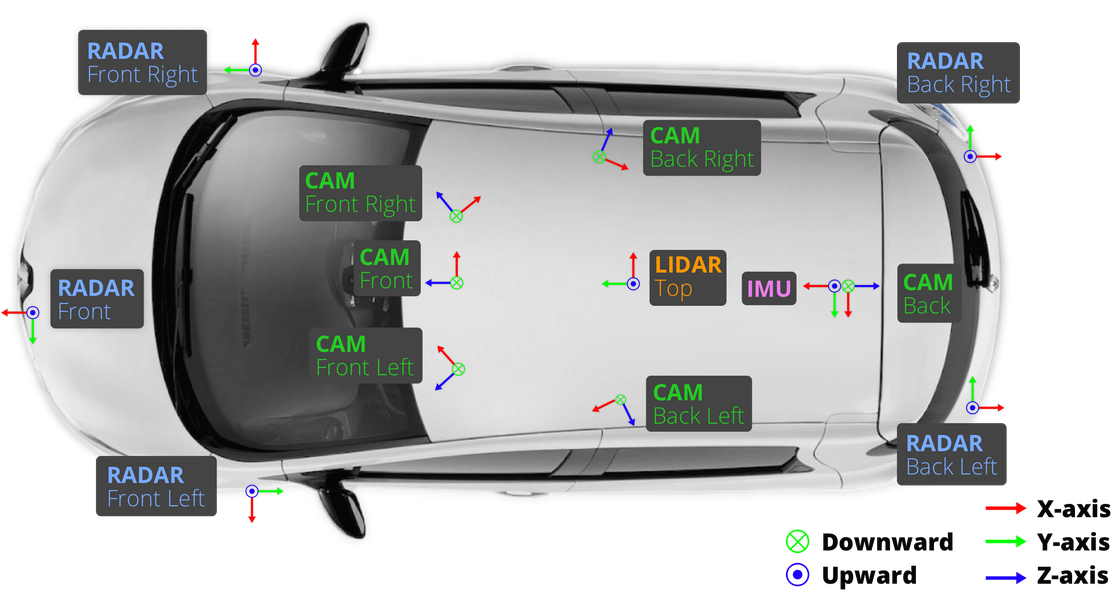
\includegraphics[width=15cm]{NuScenes_Vehicle.png}
  \caption{NuScenes autonomous vehicle sensor setup}\label{fig:AutoVehicle}
\end{figure}

The autonomous vehicle collects sensor readings from the sensors shown in \ref{fig:AutoVehicle}. As the vehicle drives around, these sensors 
run at a predetermined frequency, capturing information about the vehicle's surroundings and thus enabling it to drive safely.

\item [PS\refstepcounter{psysnum}\thepsysnum \label{Camera Images}:] A camera image taken from one of the cameras on the autonomous vehicle (taken from NuScenes \cite{caesar2020nuscenes}).
\begin{figure}[H]
  \centering
  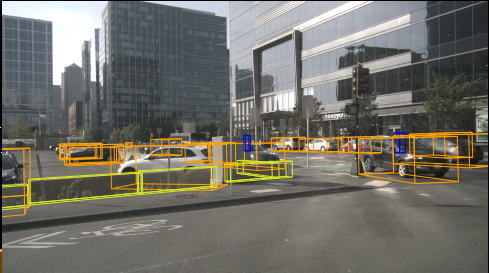
\includegraphics[width=15cm]{Camera_View.png}
  \caption{Camera image with bounding boxes taken from NuScenes}\label{fig:CameraView}
\end{figure}

The cameras on the autonomous vehicle each capture images that look similar to the image shown in \ref{fig:CameraView}. Note that while boxes are shown
in this image to highlight the other vehicles and the pedestrians in the image, the image input into the system will not have these.

\item [PS\refstepcounter{psysnum}\thepsysnum \label{LiDAR Pointclouds}:] A LiDAR pointcloud obtained from the spinning LiDAR sensor on top of the autonomous vehicle (taken from NuScenes \cite{caesar2020nuscenes}).
\begin{figure}[H]
  \centering
  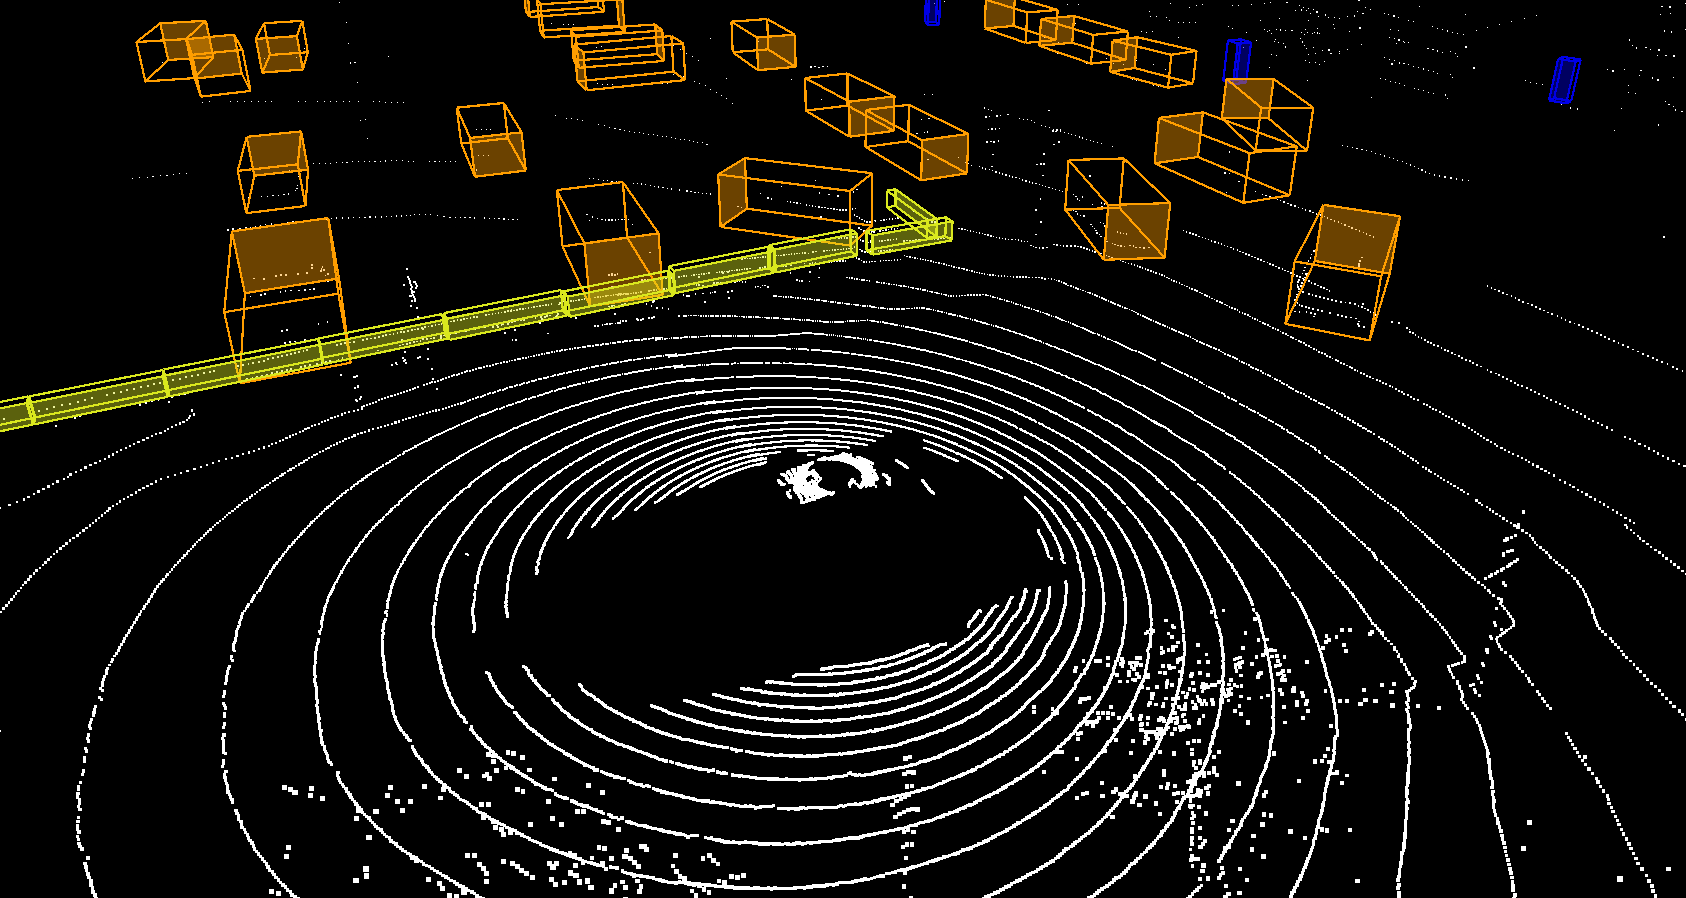
\includegraphics[width=15cm]{LiDAR_View.png}
  \caption{LiDAR pointcloud with bounding boxes taken from NuScenes}\label{fig:LiDARView}
\end{figure}

The LiDAR sensor on top of the autonomous vehicle captures information that is then converted into the pointcloud representation shown in \ref{fig:LiDARView}.
Similar to the case of the camera image shown before, the boxes in the pointcloud are for illustrative purposes and are not included in the input to the system.

\item [PS\refstepcounter{psysnum}\thepsysnum \label{Bounding Boxes}:] The bounding boxes for the a given scene in the NuScenes dataset \cite{caesar2020nuscenes}.

The LiDAR pointcloud shown in \ref{fig:LiDARView} and the camera image shown in \ref{fig:CameraView} both have boxes surrounding the vehicles,
pedestrians, and other objects of importance in the autonomous vehicle's surroundings. These boxes are called bounding boxes and they represent
the output of the system.

\end{itemize}

\subsubsection{Goal Statements}
\begin{itemize}

\item[GS\refstepcounter{goalnum}\thegoalnum \label{goal:training}:] Given a dataset comprising of multiview 
camera images with paired LiDAR pointclouds and ground-truth bounding boxes, output a model that is trained
to minimize the chosen error function on the input dataset.

\item[GS\refstepcounter{goalnum}\thegoalnum \label{goal:inference}:] Given multi-view camera images, a 
corresponding LiDAR pointcloud from an autonomous vehicle, and the trained model from GS2, output the set of bounding boxes for dynamic entities
in the autonomous vehicle's surroundings.

\end{itemize}

\subsection{Solution Characteristics Specification}

The instance models that govern \ProjectName are presented in
Subsection~\ref{sec_instance}.  The information to understand the meaning of the
instance models and their derivation is also presented, so that the instance
models can be verified.

\subsubsection{Types}

This section is not used at the moment, but it may be used in future iterations of this document.

\subsubsection{Scope Decisions}

This section is not used at the moment, but it may be used in future iterations of this document.
\subsubsection{Modelling Decisions}

This section is not used at the moment, but it may be used in future iterations of this document.

\subsubsection{Assumptions} \label{sec_assumpt}

This section simplifies the original problem and helps in developing the
theoretical model by filling in the missing information for the physical system.
The numbers given in the square brackets refer to the theoretical model [TM],
general definition [GD], data definition [DD], instance model [IM], or likely
change [LC], in which the respective assumption is used. The rationale for these
assumptions is provided in \rnref{RN:Assump}.

\begin{itemize}

\item[A\refstepcounter{assumpnum}\theassumpnum \label{assump:distortion}] The camera images
passed into the system are assumed to all be undistorted. That is to say that the camera images
are all assumed to follow the pinhole camera model. Used in \dref{GD:AP}.

\item[A\refstepcounter{assumpnum}\theassumpnum \label{assump:skew}] All the cameras aboard the
autonomous vehicle are assumed to have near-perfectly perpendicular $x$ and $y$ axes. Thus, the skew parameter
in the camera intrinsic matrix is assumed to be negligible. Used in \dref{GD:Intrin} and \lcref{LC:Skew}.

\item[A\refstepcounter{assumpnum}\theassumpnum \label{assump:avgprec}] The numerical integral of the precision over
a finite set of equally-spaced recall values is assumed to be close enough to the actual average precision value given 
that the set of recall values is sufficiently large. Used in \dref{GD:AP}.


\end{itemize}

\subsubsection{Theoretical Models}\label{sec_theoretical}

This section focuses on the general equations and laws that \ProjectName is based
on.


~\newline

\noindent
\deftheory
% #2 refname of theory
{TM:Intrin}
% #3 label
{3D Position to 2D Pixel Mapping}
% #4 equation
{
  $\begin{bmatrix}\mathbf{P_i} \\ 1\end{bmatrix}=D(\mathbf{K}\begin{bmatrix}\mathbf{P_c^*}\end{bmatrix})$, 
  $\mathbf{K}=\begin{bmatrix}
    f_x & s & c_x \\
    0 & f_y & c_y \\
    0 & 0 & 1
  \end{bmatrix}$,
  $\mathbf{P_c^*}\triangleq{}\begin{bmatrix}\frac{X_c}{Z_c} \\ \frac{Y_c}{Z_c} \\ 1\end{bmatrix}$
}
% #5 description
{
  The above equation describes how a 3D location $\mathbf{P_c}$ in the camera's reference frame 
  is mapped to a 2D location in the camera's image plane $\mathbf{P_i}$. It also shows how the
  camera's intrinsic matrix $\mathbf{K}$ used in this equation is constructed from the camera's focal 
  lengths $f_x$ and $f_y$, the camera's skew parameter $s$, and the camera's principal points $c_x$ and $c_y$. The outer 
  function $D$ represents the inherent distortion introduced due to the lens characteristics of the camera.
}
% #6 Notes
{
}
% #7 Source
{ \cite{Barfoot_2017}
}
% #8 Referenced by
{ \dref{GD:Intrin}
}
% #9 Preconditions
{
}
% #1 derivation - not applicable by default
{}

~\newline

\noindent
\deftheory
% #2 refname of theory
{TM:Extrin}
% #3 label
{Camera Extrinsics}
% #4 equation
{
  $\begin{bmatrix}\mathbf{P_w}\\1\end{bmatrix} = \mathbf{T_{c,w}}\begin{bmatrix}\mathbf{P_c}\\1\end{bmatrix}$,
  $\mathbf{T_{c,w}} = \begin{bmatrix}
  \mathbf{R_{c,w}} & \mathbf{t_{c,w}} \\
  0 & 1
  \end{bmatrix}$
}
% #5 description
{
  The above equation gives the general relation between a point's coordinates $\mathbf{P_c}$ in some original frame and its coordinates $\mathbf{P_w}$ in some other reference frame.
  It also shows how the extrinsics matrix $\mathbf{T_{c,w}}$ can be decomposed into a rotation $\mathbf{R_{c,w}}$ and a translation $\mathbf{t_{c,w}}$ between the two reference frames. 
}
% #6 Notes
{
}
% #7 Source
{ \cite{Barfoot_2017}
}
% #8 Referenced by
{ \iref{IM:CamToWorld}
}
% #9 Preconditions
{
}
% #1 derivation - not applicable by default
{}


~\newline

\noindent
\deftheory
% #2 refname of theory
{TM:CE}
% #3 label
{Categorical Cross Entropy}
% #4 equation
{
  $CE(\mathbb{P},t)=-\log(\mathbb{P}[t])$
}
% #5 description
{
  The equation above represents a loss function that is commonly used for classification tasks in machine learning.
  Given a probability distribution over the set of possible classes $\mathbb{P}$ as well as the index of the correct class $t$ ($\mathbb{R}$),
  it provides a measure of how poorly the probability distribution predicted the correct class. It penalizes larger errors (probabilities
  closer to 0) much more harshly than minor errors (probabilities closer to 1) due to the log term.
}
% #6 Notes
{
}
% #7 Source
{ \cite{ross2017focal}
}
% #8 Referenced by
{ \iref{IM:BBLoss}
}
% #9 Preconditions
{
}
% #1 derivation - not applicable by default
{}

~\newline

\noindent
\deftheory
% #2 refname of theory
{TM:GD}
% #3 label
{Gradient Descent}
% #4 equation
{
  $\mathbf{\theta} = \mathbf{\theta} - \alpha_{gd}\nabla{}L(\theta)$
}
% #5 description
{
  The above equation is the simple update rule that forms the backbone of modern machine learning.
  Given some differentiable loss function $L$ that we wish to minimize, a rate-controlling parameter 
  $\alpha$, and a set of parameters $\mathbf{\theta}$, it updates $\mathbf{\theta}$ in a way that would reduce the obtained loss $L(\mathbf{\theta})$.
}
% #6 Notes
{
}
% #7 Source
{\cite{amari1993backpropagation}
}
% #8 Referenced by
{ \iref{IM:ADAM}
}
% #9 Preconditions
{
}
% #1 derivation - not applicable by default
{}


~\newline

\noindent
\deftheory
% #2 refname of theory
{TM:IoU}
% #3 label
{Intersection over Union}
% #4 equation
{
  $IoU(A,B)=\frac{|A\bigcap{}B|}{|A\bigcup{}B|}$
}
% #5 description
{
  Given two shapes in $n$-dimensional space $A$ and $B$, the intersection over union metric ($\mathbb{R}_{\geq0}$) provides a measure of their similarity.
  It tells us how much these two shapes overlap and thus it can indicate how well of an estimation one is for the other.
}
% #6 Notes
{
}
% #7 Source
{ \cite{openpcdet2020}
}
% #8 Referenced by
{ \iref{IM:BBLoss}, \iref{IM:mAP}
}
% #9 Preconditions
{
}
% #1 derivation - not applicable by default
{}


~\newline

\noindent
\deftheory
% #2 refname of theory
{TM:Prec}
% #3 label
{Precision}
% #4 equation
{
  $P = \frac{TP}{TP+FP}$
}
% #5 description
{
  Precision $P$ ($\mathbb{R}_{\geq0}$) is a performance metric that is used in prediction tasks to determine how often a system's predictions
  are correct. It is calculated in the formula above using the number of true positives $TP$ and the number of false positives $FP$. 
}
% #6 Notes
{
}
% #7 Source
{ \cite{zhu2004recall}
}
% #8 Referenced by
{ \tref{TM:AP}
}
% #9 Preconditions
{
}
% #1 derivation - not applicable by default
{}

~\newline

\noindent
\deftheory
% #2 refname of theory
{TM:Rec}
% #3 label
{Recall}
% #4 equation
{
  $R = \frac{TP}{TP+FN}$
}
% #5 description
{
  Recall $R$ ($\mathbb{R}_{\geq0}$) is a performance metric that is used in prediction tasks to determine how often a system is able
  to detect occurrences of whatever it is predicting. It is calculated in the formula above using the number of 
  true positives $TP$ and the number of false negatives $FN$.
}
% #6 Notes
{
}
% #7 Source
{ \cite{zhu2004recall}
}
% #8 Referenced by
{ \tref{TM:AP}
}
% #9 Preconditions
{
}
% #1 derivation - not applicable by default
{}

~\newline

\noindent
\deftheory
% #2 refname of theory
{TM:AP}
% #3 label
{Average Precision}
% #4 equation
{
  $AP = \int_0^1 P(x) \, dR(x) $
}
% #5 description
{
  Average Precision $AP$ ($\mathbb{R}_{\geq0}$) is a performance metric that is used in prediction tasks to capture both recall and 
  precision into a single metric. In the above formula, the symbol $x$ is simply used to capture
  the vector of controllable parameters (each in $R$) that influence both recall and precision.
  
  A high average precision score indicates that a system can predict most actual 
  occurrences without many false predictions. In its purest form, it represents the area under a curve formed by
  plotting the precision of a system against its recall. 
}
% #6 Notes
{
}
% #7 Source
{ \cite{zhu2004recall}
}
% #8 Referenced by
{ \dref{GD:AP}
}
% #9 Preconditions
{
  \tref{TM:Prec}, \tref{TM:Rec}
}
% #1 derivation - not applicable by default
{}

~\newline

\subsubsection{General Definitions}\label{sec_gendef}

This section collects the laws and equations that will be used in building the
instance models.

~\newline

\noindent
\begin{minipage}{\textwidth}
\renewcommand*{\arraystretch}{1.5}
\begin{tabular}{| p{\colAwidth} | p{\colBwidth}|}
\hline
\rowcolor[gray]{0.9}
Number& GD\refstepcounter{defnum}\thedefnum \label{GD:Intrin}\\
\hline
Label &\bf Camera Intrinsics Projection \\
\hline
Units&pixels\\
\hline

Equation&$\begin{bmatrix}\mathbf{P_i}\\1\end{bmatrix}=\mathbf{K}\mathbf{P_c^*}$, 
  $\mathbf{K}=\begin{bmatrix}
    f_x & 0 & c_x \\
    0 & f_y & c_y \\
    0 & 0 & 1
  \end{bmatrix}$,
  $\mathbf{P_c^*}=\begin{bmatrix}\frac{X_c}{Z_c} \\ \frac{Y_c}{Z_c} \\ 1\end{bmatrix}$  \\

\hline
Description &
This relation is a simplified version of \tref{TM:Intrin}. Through assumptions \aref{assump:distortion}
and \aref{assump:skew}, the distortion function and the skew parameter have been removed from the equation.
The equation still works as described in \tref{TM:Intrin}.
\\
\hline
  Source & N/A\\
  \hline
  Ref.\ By & \iref{IM:CamToWorld} \\
  \hline
\end{tabular}
\end{minipage}\\

~\newline

\noindent
\begin{minipage}{\textwidth}
\renewcommand*{\arraystretch}{1.5}
\begin{tabular}{| p{\colAwidth} | p{\colBwidth}|}
\hline
\rowcolor[gray]{0.9}
Number& GD\refstepcounter{defnum}\thedefnum \label{GD:AP}\\
\hline
Label &\bf Numerical Average Precision Approximation \\
\hline
Units&unitless\\
\hline

Equation&$AP = \sum_{k=1}^{N}(R_k-R_{k-1})P_k$  \\

\hline
Description &
Since precision and recall cannot be expressed as direct functions of some input value, the formulation in \tref{TM:AP} is impossible to solve directly.
As such, this relation uses a numerical approximate for the integral shown in that formulation. Through assumption \aref{assump:avgprec}, this numerical
approximation can directly be used in place of the actual integral. Here, $R$ ($\mathbb{R}^{N+1}_{\geq0}$) represents a set of $N+1$ discretely sampled recall values, 
while $P$ ($\mathbb{R}^{N+1}_{\geq0}$) represents the set of $N+1$ corresponding precision values.
\\
\hline
  Source & \cite{zhu2004recall}\\
  \hline
  Ref.\ By & \iref{IM:mAP} \\
  \hline
\end{tabular}
\end{minipage}\\

\subsubsection{Data Definitions}\label{sec_datadef}

This section is not used at the moment, but it may be used in future iterations of this document.

\subsubsection{Data Types}\label{sec_datatypes}

This section is not used at the moment, but it may be used in future iterations of this document.

\subsubsection{Instance Models} \label{sec_instance}    

This section transforms the problem defined in Section~\ref{Sec_pd} into 
one which is expressed in mathematical terms. It uses concrete symbols defined 
in Section~\ref{sec_datadef} to replace the abstract symbols in the models 
identified in Sections~\ref{sec_theoretical} and~\ref{sec_gendef}.

~\newline

%Instance Model 1

\noindent
\begin{minipage}{\textwidth}
\renewcommand*{\arraystretch}{1.5}
\begin{tabular}{| p{\colAwidth} | p{\colBwidth}|}
  \hline
  \rowcolor[gray]{0.9}
  Number& IM\refstepcounter{instnum}\theinstnum \label{IM:CamToWorld}\\
  \hline
  Label& \bf Camera to Reference Frame Transformation\\
  \hline
  Input&$\mathbf{K}$, $\mathbf{T_{c,w}}$, $\mathbf{d_c}$, $\mathbf{P_i}$\\
  \hline
  Output&$\mathbf{P_w}$\\
  \hline
  Description&By combining \tref{TM:Extrin} and \dref{GD:Intrin}, we can get the following equation: \\
  &$\begin{bmatrix}\mathbf{P_w}\\1\end{bmatrix}=\mathbf{T_{c,w}}\begin{bmatrix}\mathbf{K} & 0 \\ 0 & 1\end{bmatrix}^{-1}\begin{bmatrix}\begin{bmatrix}\mathbf{P_i}\\1\end{bmatrix}\circ{}\mathbf{d_c} \\ 1\end{bmatrix}$ \\
  &$\mathbf{P_w}$ represents a matrix of 3D points back-projected from the set of 2D pixel coordinates $\mathbf{P_i}$ and their corresponding depth estimates $\mathbf{d_c}$. Note that multiplying by the depth estimates here is the inverse operation to dividing by $z$ when going from 3D to 2D (as seen in \dref{GD:Intrin}).\\
  &This allows for 2D camera features to then be projected to 3D locations so that they can be merged with LiDAR. \\ 
  \hline
  Sources& N/A\\
  \hline
  Ref.\ By & \\
  \hline
\end{tabular}
\end{minipage}\\

~\newline

%Instance Model 1

\noindent
\begin{minipage}{\textwidth}
\renewcommand*{\arraystretch}{1.5}
\begin{tabular}{| p{\colAwidth} | p{\colBwidth}|}
  \hline
  \rowcolor[gray]{0.9}
  Number& IM\refstepcounter{instnum}\theinstnum \label{IM:BBLoss}\\
  \hline
  Label& \bf Bounding Box Loss Function $L$\\
  \hline
  Input&$\mathbf{\hat{B}}$, $\mathbf{B}$, $\mathbf{\hat{C}_{\text{dist}}}$, $\mathbf{c}$, $\alpha_{fl}$, $\gamma$\\
  \hline
  Output&$RL$, $FL$, $L$\\
  \hline
  Description&Given the set of predicted bounding boxes $\mathbf{\hat{B}}$ and the set of ground-truth bounding boxes $\mathbf{B}$,
  the set of paired ground-truth bounding boxes $\mathbf{B^{*}}$ and paired ground-truth bounding box classes $\mathbf{c^{*}}$ will be defined as follows using the IoU function defined in \tref{TM:IoU}:\\
  &$\mathbf{B^{*}}[,i]=\mathbf{B}[,\arg\max_j \text{IoU}(\mathbf{\hat{B}}[,i],\mathbf{B}[,j])]$,\\& $\mathbf{c^*}[i]=\mathbf{c}[\arg\max_j \text{IoU}(\mathbf{\hat{B}}[,i],\mathbf{B}[,j])]$\\
  &Then, by using the predicted-ground truth bounding box pairings, the regression loss can be defined as follows:\\
  &$RL(\mathbf{\hat{B}}, \mathbf{B^{*}})=\sum_{k=0}^{n_{\hat{b}}-1}\frac{|\mathbf{\hat{B}}[,k]-\mathbf{B^*}[,k]|}{n}$\\
  &While this penalizes predicted boxes being far from ground truth boxes, an additional loss term is needed to ensure that boxes are classified correctly. As such, a focal classification loss using the paired ground truth bounding box classes can be defined as follows:\\
  &$FL(\mathbf{\hat{C}_{\text{dist}}}, \mathbf{c^{*}})=-\sum_{k=0}^{n_{\hat{b}}-1}\alpha_{fl}(1-\mathbf{\hat{C}_{\text{dist}}}[\mathbf{c^{*}}[k], k])^{\gamma}\log{}(\mathbf{\hat{C}_{\text{dist}}}[\mathbf{c^{*}}[k], k])$\\
  &This function is derived from the cross-entropy equation \tref{TM:CE}, with an additional term to downweight easy examples. \\
  &By combining the regression loss with the classification loss, the total bounding box loss function (to be used for optimization) can be defined as follows:\\
  &$L(\mathbf{\hat{B}}, \mathbf{B^{*}}, \mathbf{\hat{C}_{\text{dist}}}, \mathbf{c^{*}}) = RL(\mathbf{\hat{B}}, \mathbf{B^{*}}) + FL(\mathbf{\hat{C}_{\text{dist}}}, \mathbf{c^{*}})$\\
  \hline
  Sources&\cite{ross2017focal}, \cite{openpcdet2020}\\
  \hline
  Ref.\ By & \iref{IM:ADAM} \\
  \hline
\end{tabular}
\end{minipage}\\

~\newline

%Instance Model 1

\noindent
\begin{minipage}{\textwidth}
\renewcommand*{\arraystretch}{1.5}
\begin{tabular}{| p{\colAwidth} | p{\colBwidth}|}
  \hline
  \rowcolor[gray]{0.9}
  Number& IM\refstepcounter{instnum}\theinstnum \label{IM:ADAM}\\
  \hline
  Label& \bf Model Training via ADAM Optimization $T_W$\\
  \hline
  Input&$\theta_{t}$, $\beta_1$, $\beta_2$, $\alpha_{gd}$\\
  \hline
  Output&$\theta_{t+1}$\\
  \hline
  Description&With the loss function established in \iref{IM:BBLoss}, a gradient-based method for updating a chosen system's parameters $\mathbf{\theta_{t}}$ can be setup as follows: \\
  &$\mathbf{g_t}=\nabla_{\mathbf{\theta}}L(\mathbf{\theta_t})$\\
  &Where gradient descent \tref{TM:GD} would simply subtract off this gradient to update the parameters $\mathbf{\theta_t}$, a modified form inspired by statistical moments can be used instead (called ADAM): \\
  &$\mathbf{m_{t}} = \beta_1\mathbf{m_{t-1}} + (1-\beta_1)\mathbf{g_t}$\\
  &$\mathbf{v_{t}} = \beta_2\mathbf{v_{t-1}} + (1-\beta_2)\mathbf{g_t}^2$\\
  &$\mathbf{\hat{m}_{t}} = \frac{\mathbf{m_{t}}}{1-\beta_1^t}$\\
  &$\mathbf{\hat{v}_{t}} = \frac{\mathbf{v_{t}}}{1-\beta_2^t}$\\
  &$\mathbf{\theta_{t+1}}=\mathbf{\theta_{t}}-\alpha_{gd}\frac{\mathbf{\hat{m}_t}}{\sqrt{\mathbf{\hat{v}_t}}+10^{-8}}$\\
  &This optimization process in conjuction with the aforementioned loss function forms the backbone of the training pipeling.\\
  \hline
  Sources&\cite{kingma2014adam}\\
  \hline
  Ref.\ By &\\
  \hline
\end{tabular}
\end{minipage}\\

~\newline

%Instance Model 1

\noindent
\begin{minipage}{\textwidth}
\renewcommand*{\arraystretch}{1.5}
\begin{tabular}{| p{\colAwidth} | p{\colBwidth}|}
  \hline
  \rowcolor[gray]{0.9}
  Number& IM\refstepcounter{instnum}\theinstnum \label{IM:mAP}\\
  \hline
  Label& \bf Model Evaluation via Mean Average Precision\\
  \hline
  Input&$\mathbf{\hat{B}}$, $\mathbf{B}$, $\mathbf{\hat{c}}$, $\mathbf{c}$, $\tau_{IoU}$\\
  \hline
  Output&$\text{mAP}$\\
  \hline
  Description&Using the classes for the predicted bounding boxes $\mathbf{\hat{c}}$ and the classes for the ground-truth bounding boxes $\mathbf{c}$, their corresponding bounding box sets can be partitioned into class-specific bounding boxes as follows:\\
  &$\mathbf{\hat{B}^{c}} = \{\mathbf{\hat{B}}[,i] | \mathbf{\hat{c}}[i]=c\}$ and $\mathbf{B^{c}}=\{\mathbf{B}[,i] | \mathbf{c}[i]=c\}$, for all possible classes $c$ \\
  &Then, the true positives $TP$, false positives $FP$, and false negatives $FN$ for a class can be defined as follows by using the IoU metric described in \tref{TM:IoU}: \\
  &$TP(\mathbf{\hat{B}^{c}},\mathbf{B^{c}})=\sum_{k=0}^{n_{\hat{b}}-1}\max_{i}1((\text{IoU}(\mathbf{\hat{B}^c}[,k],\mathbf{B^c}[,i]))\geq{}\tau_{IoU})$\\
  &$FP(\mathbf{\hat{B}^{c}},\mathbf{B^{c}})=\sum_{k=0}^{n_{\hat{b}}-1}(1-\max_{i}1((\text{IoU}(\mathbf{\hat{B}^c}[,k],\mathbf{B^c}[,i]))\geq\tau_{IoU}))=n_{\hat{b}}-TP$\\
  &$FN(\mathbf{\hat{B}^{c}},\mathbf{B^{c}})=\sum_{k=0}^{n_{b}-1}(1-\max_{i}1((\text{IoU}(\mathbf{B^c}[,k],\mathbf{\hat{B}^c}[,i]))\geq\tau_{IoU}))$\\
  &Using these values, the average precision values for each class can be calculate as described in \dref{GD:AP}. The final $mAP$ metric is then calculated by averaging these as follows:\\
  &$\text{mAP}(\mathbf{\hat{B}}, \mathbf{B}, \mathbf{\hat{c}}, \mathbf{c})=\sum_{c}\frac{AP(\mathbf{\hat{B}^{c}},\mathbf{B^{c}})}{|c|}$\\
  \hline
  Sources&\cite{openpcdet2020}\\
  \hline
  Ref.\ By &\\
  \hline
\end{tabular}
\end{minipage}\\

\subsubsection{Input Data Constraints} \label{sec_DataConstraints}    

Table~\ref{TblInputVar} shows the data constraints on the input output
variables.  The column for physical constraints gives the physical limitations
on the range of values that can be taken by the variable.  The column for
software constraints restricts the range of inputs to reasonable values.  The
software constraints will be helpful in the design stage for picking suitable
algorithms.  The constraints are conservative, to give the user of the model the
flexibility to experiment with unusual situations.  The column of typical values
is intended to provide a feel for a common scenario.  The uncertainty column
provides an estimate of the confidence with which the physical quantities can be
measured.  This information would be part of the input if one were performing an
uncertainty quantification exercise.

The specification parameters in Table~\ref{TblInputVar} are listed in
Table~\ref{TblSpecParams}.

\begin{table}[!h]
  \caption{Input Variables} \label{TblInputVar}
  \renewcommand{\arraystretch}{1.2}
\noindent \begin{longtable*}{l l l l c} 
  \toprule
  \textbf{Var} & \textbf{Physical Constraints} & \textbf{Software Constraints} &
                             \textbf{Typical Value} & \textbf{Uncertainty}\\
  \midrule 
  $p_{i,j}$ & - & $p_{\text{min}} \leq p_{i,j} \leq p_{\text{max}}$ & Any valid value & Unknown
  \\
  $w$ & $w\geq0$ & $w_{\text{min}} \leq w \leq w_{\text{max}}$ & 1920 pixels & Unknown
  \\
  $h$ & $h\geq0$ & $h_{\text{min}} \leq h \leq h_{\text{max}}$ & 1280 pixels & Unknown
  \\
  \bottomrule
\end{longtable*}
\end{table}

\noindent 

\begin{table}[!h]
\caption{Specification Parameter Values} \label{TblSpecParams}
\renewcommand{\arraystretch}{1.2}
\noindent \begin{longtable*}{l l} 
  \toprule
  \textbf{Var} & \textbf{Value} \\
  \midrule 
  $p_\text{min}$ & 0\\
  $p_\text{min}$ & 255\\
  $w_\text{min}$ & 24\\
  $w_\text{min}$ & 4096\\
  $h_\text{min}$ & 24\\
  $h_\text{min}$ & 4096\\
  \bottomrule
\end{longtable*}
\end{table}

\subsubsection{Properties of a Correct Solution} \label{sec_CorrectSolution}

Rather than describe the properties of a correct solution in a table, I think It
is more illustrative to describe them in words. The main properties of a correct solution in inference
are that output bounding boxes must be non-overlapping and must have positive width, length, and height.

\section{Requirements}

This section provides the functional requirements, the business tasks that the
software is expected to complete, and the nonfunctional requirements, the
qualities that the software is expected to exhibit.

\newpage

\subsection{Functional Requirements}

\noindent \begin{itemize}

\item[R\refstepcounter{reqnum}\thereqnum \label{Req:CamIn}:] During inference, input images should be accepted in the following formats:
\begin{itemize}
  \item PNG (Portable Net Graphics)
  \item JPEG (Joint Photographic Experts Group)
  \item TFRecord (TensorFlow Binary Record)
  \item PT (Pytorch Tensor File)
\end{itemize}

\item[R\refstepcounter{reqnum}\thereqnum \label{Req:LiDARIn}:] During inference, input LiDAR pointclouds should be accepted in the following formats:
\begin{itemize}
  \item PCD (Point Cloud Data)
  \item PLY (Polygon File Format)
  \item TFRecord (TensorFlow Binary Record)
  \item PT (Pytorch Tensor File)
\end{itemize}

\item[R\refstepcounter{reqnum}\thereqnum \label{Req:Optim}:] Given an input dataset, the system shall be designed to output a trained model that minimizes 
the combined bounding box loss \iref{IM:BBLoss} on the training subset using the ADAM optimization method \iref{IM:ADAM}. 

\item[R\refstepcounter{reqnum}\thereqnum \label{Req:Vis}:] In inference, the system shall predict the set of dynamic object bounding boxes and visualize
them on the LiDAR pointcloud that was inputted in.

\end{itemize}

\subsection{Nonfunctional Requirements}
\noindent \begin{itemize}

\item[NFR\refstepcounter{nfrnum}\thenfrnum \label{NFR:Accuracy}:]
  \textbf{Accuracy} The accuracy of the software shall be measured using the mAP metric \iref{IM:mAP}. The level of accuracy achieved
  by \ProjectName shall be comparable to that of the BEVFusion method \cite{liang2022bevfusion} presented in the OpenPCDet repository \cite{openpcdet2020} (on the NuScenes \cite{caesar2020nuscenes} or Waymo \cite{sun2020scalability} dataset). 

\item[NFR\refstepcounter{nfrnum}\thenfrnum \label{NFR:Understandability}:]
  \textbf{Understandability} As \ProjectName is meant to be modified and used for research purposes,
    the classes and functions designed in \ProjectName shall be fully documented in a way that minimizes the effort needed
    for a domain expert to understand them.

\item Maintainability and Portability are inherited from the greater OpenPCDet repository \cite{openpcdet2020} and thus are not explicitly considered.

\end{itemize}

\subsection{Rationale}

This section provides rationales for the system constraints and assumptions as follows:
\begin{itemize}
  \item[RN\refstepcounter{rnnum}\thernnum\label{RN:Learn}:] \textbf{Rationale for \cref{C1}}: For this project, I decided to focus on learned methods specifically because I have seen learned methods for this task often presented at scientific conferences. 
  Additionally, my main area of focus is in deep learning for computer vision, so I also chose this constraint to match my interests. With this in mind, OpenPCDet \cite{openpcdet2020} simplifies the process of setting up datasets and 
  building models as it has much of the foundational code fully setup so its use was a logical constraint to make the problem more tractable in the 3 months of the term. It also provides implementations and benchmark
  values for reference methods like BEVFusion \cite{liang2022bevfusion}, so it simplifies evaluation and verification of \nfrref{NFR:Accuracy} as well.
  \item[RN\refstepcounter{rnnum}\thernnum\label{RN:Dataset}:] \textbf{Rationale for \cref{C2}}: Reference methods for this task are often evaluated on these benchmark datasets so enforcing their use simplifies the evaluation of \nfrref{NFR:Accuracy}.
  \item[RN\refstepcounter{rnnum}\thernnum\label{RN:Optim}:] \textbf{Rationale for \cref{C3}}: Reference methods for this task are almost always trained with the ADAM optimizer, so allowing the use of other optimizers would simply add more complexity and ambiguity to the results obtained.
  \item[RN\refstepcounter{rnnum}\thernnum\label{RN:Assump}:] \textbf{Rationale for \aref{assump:distortion}, \aref{assump:skew}, \aref{assump:avgprec}}: These assumptions are commonly made in open-source libraries like OpenPCDet \cite{openpcdet2020}, so it makes sense to have them for this project as well.
\end{itemize}

\section{Likely Changes}    

\noindent \begin{itemize}
\item[LC\refstepcounter{lcnum}\thelcnum\label{LC:Loss}:] While the loss functions presented are commonly used and thus are unlikely to be removed, the greater loss function may have additional terms incorporated in \iref{IM:BBLoss}.
\item[LC\refstepcounter{lcnum}\thelcnum\label{LC:Skew}:] Depending on the dataset used for training and the data used for inference, the skew parameter in the intrinsic matrix may need to be considered \aref{assump:skew}.
\end{itemize}

\section{Unlikely Changes}    

\noindent \begin{itemize}

\item[ULC\refstepcounter{ulcnum}\theulcnum\label{ULC:meaningfulLabel}:] The choice of ADAM as the optimization algorithm is unlikely to change as it allows for an easier comparison to state-of-the-art methods.

\end{itemize}

\section{Traceability Matrices and Graphs}

The purpose of the traceability matrices is to provide easy references on what
has to be additionally modified if a certain component is changed.  Every time a
component is changed, the items in the column of that component that are marked
with an ``X'' may have to be modified as well.  Table~\ref{Table:trace} shows the
dependencies of theoretical models, general definitions, data definitions, and
instance models with each other. Table~\ref{Table:R_trace} shows the
dependencies of instance models, requirements, and data constraints on each
other. Table~\ref{Table:A_trace} shows the dependencies of theoretical models,
general definitions, data definitions, instance models, and likely changes on
the assumptions.

\begin{landscape}
\begin{table}[h!]
\centering
\scalebox{0.8}{
\begin{tabular}{|c|c|c|c|c|c|c|c|c|c|c|c|c|c|c|}
\hline
	& \tref{TM:Intrin} & \tref{TM:Extrin}& \tref{TM:CE}& \tref{TM:GD}& \tref{TM:IoU}& \tref{TM:Prec}& \tref{TM:Rec}& \tref{TM:AP}& \dref{GD:Intrin}& \dref{GD:AP}& \iref{IM:CamToWorld}& \iref{IM:BBLoss}& \iref{IM:ADAM}& \iref{IM:mAP}\\
\hline
\tref{TM:Intrin}        & & & & & & & & & & & & & & \\ \hline
\tref{TM:Extrin}        & & & & & & & & & & & & & & \\ \hline
\tref{TM:CE}            & & & & & & & & & & & & & & \\ \hline
\tref{TM:GD}            & & & & & & & & & & & & & & \\ \hline
\tref{TM:IoU}           & & & & & & & & & & & & & & \\ \hline
\tref{TM:Prec}          & & & & & & & & & & & & & & \\ \hline
\tref{TM:Rec}           & & & & & & & & & & & & & & \\ \hline
\tref{TM:AP}            & & & & & &X&X& & & & & & & \\ \hline
\dref{GD:Intrin}        &X& & & & & & & & & & & & & \\ \hline
\dref{GD:AP}            & & & & & &X&X&X& & & & & & \\ \hline
\iref{IM:CamToWorld}    &X&X& & & & & & &X& & & & & \\ \hline
\iref{IM:BBLoss}        & & &X& &X& & & & & & & & & \\ \hline
\iref{IM:ADAM}          & & & &X& & & & & & & &X& & \\ \hline
\iref{IM:mAP}           & & & & &X&X&X&X& &X& & & & \\ 
\hline
\end{tabular}}
\caption{Traceability Matrix Showing the Connections Between Items of Different Sections}
\label{Table:trace}
\end{table}
\end{landscape}

\begin{table}[h!]
\centering
\begin{tabular}{|c|c|c|c|c|c|c|c|c|c|c|c|}
\hline
	& \iref{IM:CamToWorld}& \iref{IM:BBLoss}& \iref{IM:ADAM}& \iref{IM:mAP}& \ref{sec_DataConstraints}& \rref{Req:CamIn}& \rref{Req:LiDARIn}& \rref{Req:Optim}& \rref{Req:Vis}& \nfrref{NFR:Accuracy}& \nfrref{NFR:Understandability} \\
\hline
\iref{IM:CamToWorld}             & & & & &X& & & & & & \\ \hline
\iref{IM:BBLoss}                 & & & & & & & & & & & \\ \hline
\iref{IM:ADAM}                   & &X& & & & & & & & & \\ \hline
\iref{IM:mAP}                    & & & & & & & & & & & \\ \hline
\ref{sec_DataConstraints}        & & & & & & & & & & & \\ \hline
\rref{Req:CamIn}                 & & & & &X& & & & & & \\ \hline
\rref{Req:LiDARIn}               & & & & & & & & & & & \\ \hline
\rref{Req:Optim}                 & &X&X& & & & & & & & \\ \hline
\rref{Req:Vis}                   & & & & & & & & & & & \\ \hline 
\nfrref{NFR:Accuracy}            & & & &X& & & & & & & \\ \hline
\nfrref{NFR:Understandability}   & & & & & & & & & & & \\
\hline
\end{tabular}
\caption{Traceability Matrix Showing the Connections Between Requirements and Instance Models}
\label{Table:R_trace}
\end{table}

\begin{table}[h!]
\centering
\begin{tabular}{|c|c|c|c|}
\hline
	& \aref{assump:avgprec} & \aref{assump:distortion}& \aref{assump:skew}\\
\hline
\dref{GD:Intrin}        & &X&X\\ \hline
\dref{GD:AP}            &X& & \\ \hline
\iref{IM:CamToWorld}    & &X&X\\ \hline
\iref{IM:BBLoss}        & & & \\ \hline
\iref{IM:ADAM}          & & & \\ \hline
\iref{IM:mAP}           &X& & \\ 
\hline
\end{tabular}
\caption{Traceability Matrix Showing the Connections Between Assumptions and Other Items}
\label{Table:A_trace}
\end{table}

\section{Development Plan}

This section is not used at the moment, but it may be used in future iterations of this document.

\section{Values of Auxiliary Constants}

This section is not used at the moment, but it may be used in future iterations of this document.

\newpage

\bibliographystyle {plainnat}
\bibliography {../../refs/References}

\newpage

\end{document}